\section{Hardware-Software-Codesign}

\subsection{Ziele}

\begin{itemize}
    \item Entwurf (Design) \textbf{so lange wie sinnvoll} (nicht so lange wie möglich) \textbf{lösungsneutral}
    \item \textbf{Systemdesign fördern}, statt separate Designs für Mechanik, Elektronik, Firmware, Software, etc., die sich
        unter Umständen auch widersprechen können
    \item Systemspezifikation erfolgt idealerweise mit Hilfe einer \textbf{eindeutigen Spezifikationssprache}, nicht in
        Prosa
    \item Die Spezifikation sollte simuliert (ausgeführt) werden können
    \item Implementationen können einfach geändert werden: HW \textlrarrow\ SW
    \item Zielplattformen: diskrete Elektronik, ASIC, \micro C, DSP, \textbf{FPGA}, Software
\end{itemize}


\subsection{Anforderungen für praktische Anwendungen}

\begin{outline}
    \1 Methoden / Tools sollten beim Systemdesign nicht zu fachlastig sein
        \2 Methoden sollten für Elektronik-, Firmware- und wenn möglich auch Mechanikentwickler anwendbar sein
    \1 Wenn möglich gute Toolunterstützung
    \1 (Automatische Synthese aus dem Modell)
\end{outline}


\subsection{Spezifikationssprachen}

\begin{minipage}[t]{0.48\columnwidth}
    \raggedright
    \begin{itemize}
    \item \textbf{Formale Sprachen sind eindeutig} \\
        (Prosa immer mehrdeutig)
    \item Spezifikation kann compiliert und ausgeführt werden \textrightarrow\ Simulationen
    \item Die ausführbare Spezifikation dient als \textbf{Golden Reference} für die künftigen Entwicklungsschritte
\end{itemize}
\end{minipage}
\hfill
\begin{minipage}[t]{0.48\columnwidth}
    \myul{\textbf{Beispiele für Spezifikationssprachen}}

    \vspace{0.1cm}

    \begin{itemize}
        \item SystemC (eine C++-Template Library)
        \item SysML
        \item SpecC
        \item SystemVerilog
        \item Esterel
        \item Matlab/Simulink
        \item Statecharts
    \end{itemize}
\end{minipage}


\subsection{Virtuelle Prototypen}

\begin{itemize}
    \item Die Simulation des Systems kann unterschiedlich stark detailliert werden
    \item \textbf{Die simulierten Systeme sind Virtuelle Prototypen}
    \item Während der Entwicklung können einzelne (virtuelle) Teile des Prototyps laufend durch physische Teile
        ersetzt werden
\end{itemize}


\subsection{X-in-the-loop}

\begin{outline}
    \1 \textbf{Model-in-the-Loop (MIL):} vollständig als Modell vorliegender virtuellen Prototyp
    \1 Je mehr der Prototyp durch konkretere Implementationen ersetzt wird, spricht man von
        \2 Software-in-the loop (SIL)
        \2 Processor-in-the loop (PIL)
        \2 Hardwarein-the loop (HIL)
\end{outline}

\vspace{0.2cm}

\textrightarrow\ Test outputs werden jeweils mit \textbf{Golden Reference} verglichen
\begin{center}
    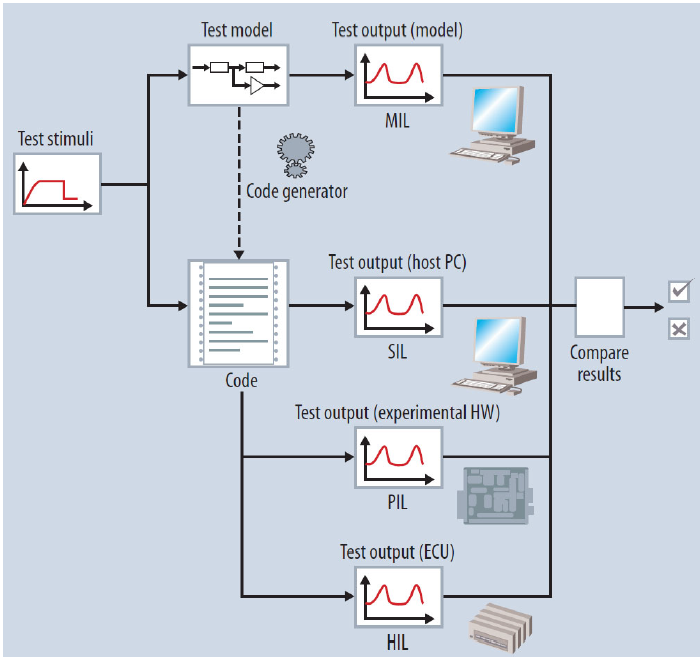
\includegraphics[width=0.9\columnwidth]{images/x_in_loop_testing.png}
\end{center}


\subsection{Entwicklungsplattformen}

Als Entwicklungsplattformen eignen sich häufig \textbf{FPGA basierte Systeme.}

\begin{outline}
    \1 Hardware mit VHDL
    \1 Software/Firmware in C/C++
        \2 auf integriertem \micro C (z.B. Zynq von AMD/Xilinx) (Hard core)
        \2 auf Soft Core innerhalb FPGA (z.B. Nios II von Intel/Altera)
\end{outline}

